

\actTitle{Worksheet 1.7}

\noindent \textbf{Instructions:} Work together in groups of 3 or 4 to
complete the following problems.

\noindent
Student goals:
  \begin{itemize}
  \item Determine if a \textbf{simple} function is an even or odd
    function given a graphical representation or algebraic expression.
  \item Define piecewise defined functions with correct notation.
  \item Graph a function defined using piecewise defined notation.
  \item Identifying the subset of a domain where a function is increasing, decreasing, or is constant.
  \item Determine relative minima and maxima from a graphical
    representation or for the algebraic representation of simple
    functions.
  \end{itemize}



\begin{enumerate}
\item Graph each of the following piecewise functions.
\begin{enumerate}
\item \[
  f(x) =
  \begin{cases}
                                   x+5 & \text{if $x<-2$} \\
                                   -4 & \text{if $x \geq 2$}

  \end{cases}
\]

\begin{center}
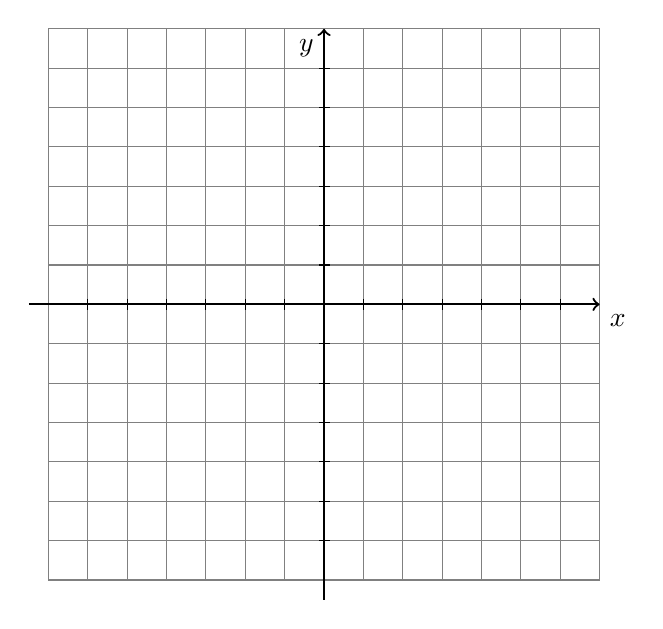
\begin{tikzpicture}[y=.5cm, x=0.5cm,font=\sffamily]
    %% ticks
    \draw[step = 1, gray] (-7,-7) grid (7,7);
    %% axis
    \draw[thick,->] (-7.5,0) -- coordinate (x axis mid) (7,0) node[anchor = north west] {$x$};
    \draw[thick,->] (0,-7.5) -- coordinate (y axis mid) (0,7) node[anchor = north east] {$y$};
    \foreach \y in {-6,-5,...,-1,1,2,...,6} {
      \draw (2pt, \y) -- (-2pt, \y);
    }
    \foreach \x in {-6,-5,...,-1,1,2,...,6} {
      \draw (\x,2pt) -- (\x,-2pt);
    }

\end{tikzpicture}
\end{center}  

\clearpage

\item \[
  f(x) =
  \begin{cases}
                                   2x+1 & \text{if $x<1$} \\
                                   -2x+3 & \text{if $x \geq 1$}

  \end{cases}
\]

\begin{center}
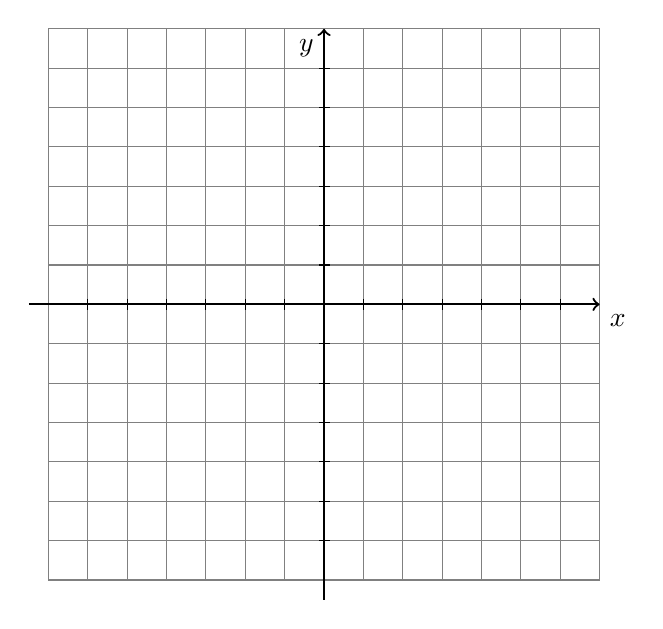
\begin{tikzpicture}[y=.5cm, x=0.5cm,font=\sffamily]
    %% ticks
    \draw[step = 1, gray] (-7,-7) grid (7,7);
    %% axis
    \draw[thick,->] (-7.5,0) -- coordinate (x axis mid) (7,0) node[anchor = north west] {$x$};
    \draw[thick,->] (0,-7.5) -- coordinate (y axis mid) (0,7) node[anchor = north east] {$y$};
    \foreach \y in {-6,-5,...,-1,1,2,...,6} {
      \draw (2pt, \y) -- (-2pt, \y);
    }
    \foreach \x in {-6,-5,...,-1,1,2,...,6} {
      \draw (\x,2pt) -- (\x,-2pt);
    }

\end{tikzpicture}
\end{center}


\item \[
  f(x) =
  \begin{cases}
                                   5 & \text{if $x<-2$} \\
                                   \frac{1}{2} & \text{if $-2 \leq x \leq 6$}\\
                                   -2x+10 & \text{if $x > 6$}

  \end{cases}
\]

\begin{center}
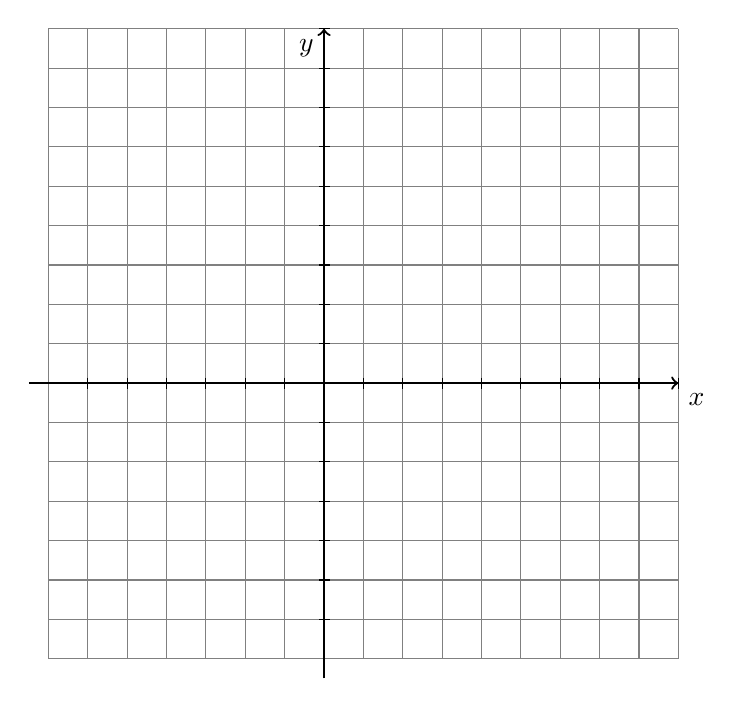
\begin{tikzpicture}[y=.5cm, x=0.5cm,font=\sffamily]
    %% ticks
    \draw[step = 1, gray] (-7,-7) grid (9,9);
    %% axis
    \draw[thick,->] (-7.5,0) -- coordinate (x axis mid) (9,0) node[anchor = north west] {$x$};
    \draw[thick,->] (0,-7.5) -- coordinate (y axis mid) (0,9) node[anchor = north east] {$y$};
    \foreach \y in {-6,-5,...,-1,1,2,...,9} {
      \draw (2pt, \y) -- (-2pt, \y);
    }
    \foreach \x in {-6,-5,...,-1,1,2,...,9} {
      \draw (\x,2pt) -- (\x,-2pt);
    }

\end{tikzpicture}
\end{center}

\end{enumerate}

\clearpage

\item Evaluate the piecewise function for the given values of $x$.
\begin{enumerate}
\item \[
  f(x) =
  \begin{cases}
                                   x+5 & \text{if $x<-2$} \\
                                   -4 & \text{if $x \geq 2$}

  \end{cases}
\]

$$f(3)= \quad \quad \quad \quad \quad \quad \quad \quad \quad \quad \quad \quad f(-4)= \quad \quad \quad \quad \quad \quad \quad \quad \quad \quad  f(-2)=\quad \quad$$

\item \[
  f(x) =
  \begin{cases}
                                   x-1 & \text{if $x<-2$} \\
                                   2x-1 & \text{if $-2< x \leq 4$}\\
                                   -3x+8 & \text{if $x>4$}

  \end{cases}
\]

$$f(-1)= \quad \quad \quad \quad \quad \quad \quad \quad \quad \quad \quad \quad f(-4)= \quad \quad \quad \quad \quad \quad \quad \quad \quad \quad f(5)=\quad \quad $$



\end{enumerate}

\item For each of the following functions, determine if the function
  is even, odd, or neither. (Show your work and justify your
  conclusion using the relevant definitions.)
\begin{enumerate}
\item $f(x)=4x^2-3|x|$
\vfill
\item $f(x)=4x^3-2x$
\vfill
\item $f(x)=4x^2+2x-3$
\vfill
\end{enumerate}

\newpage

\item Part of the graph of $f(x)$ is shown below. The graph for positive values of $x$ is shown while the portion of the graph for negative values of $x$ is missing.

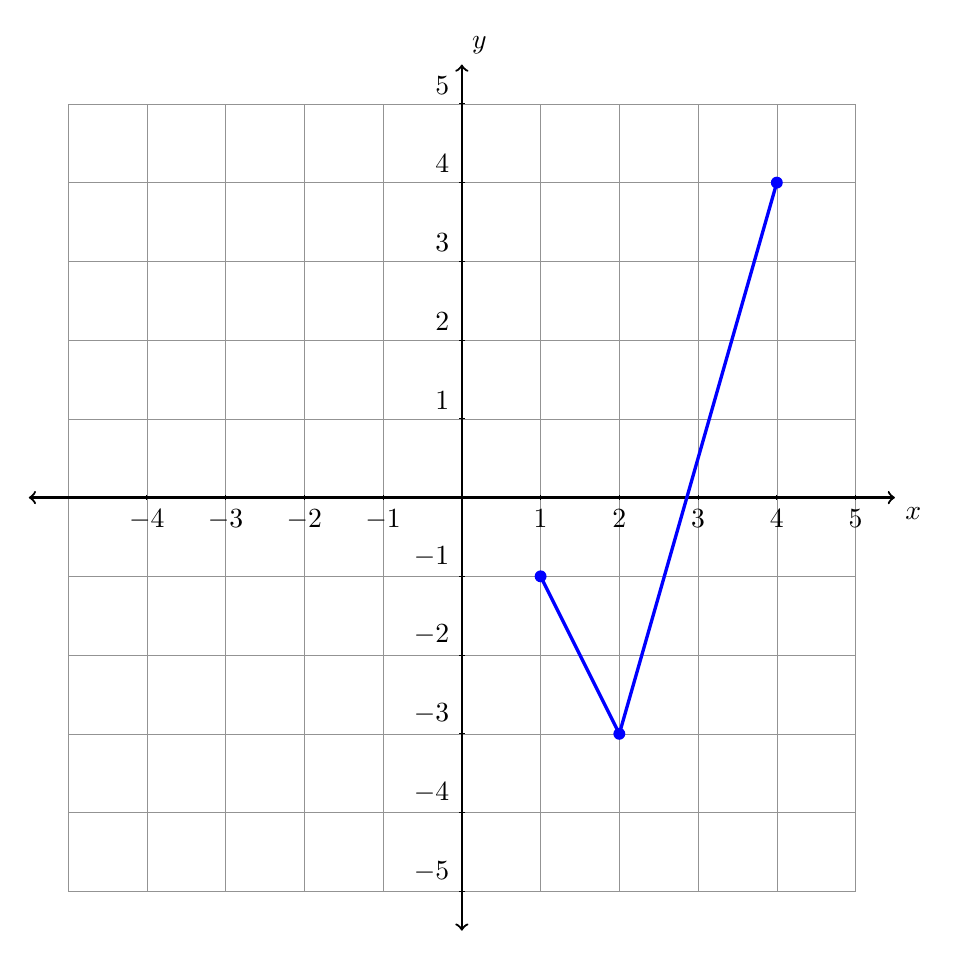
\begin{tikzpicture}[y=1cm, x=1cm,font=\sffamily,
	mydot/.style={
    circle,
    fill=white,
    draw,
    outer sep=0pt,
    inner sep=1.5pt
  }]
    %% Add a grid
    \draw[step = 1, gray, very thin,opacity=0.85] (-5, -5) grid (5, 5);
 	%% Draw the axes
	\draw[thick,<->] (-5.5,0) -- coordinate (x axis mid) (5.5,0) node[anchor = north west] {$x$};
    \draw[thick,<->] (0,-5.5) -- coordinate (y axis mid) (0,5.5) node[anchor = south west] {$y$};
    %% Label the y axis
    \foreach \y in {-5,...,-1,1,2,...,5} {
      \draw (1pt, \y) -- (-1pt, \y) node[anchor = south east] {$\y$};
    }
    %% Label the x axis
    \foreach \x in {-4,...,-1,1,2,...,5} {
      \draw (\x,1pt) -- (\x,-1pt) node[anchor = north] {$\x$};
    }
    %% Draw the function.
    \begin{scope}
         \draw[very thick,blue] (1,-1) -- (2,-3) -- (4,4);
     
    %semi-circle
         %\draw[very thick, blue] (1,1) arc [radius=1, start angle=180, end angle= 5];
     %parabola
     %    \draw[ultra thick, blue, domain=-5:0] plot (\x, {(-0.2)*(\x-5)*(\x+5)});
     %dots
         \fill[blue] (1,-1) circle[radius=0.5ex];
         \fill[blue] (2,-3) circle[radius=0.5ex];
         \fill[blue] (4,4) circle[radius=0.5ex];
      


    \end{scope}

    %%\node[above=0.1cm] at (-2,2 )   {\nextXValue};

\end{tikzpicture}





\begin{enumerate}
	\item Sketch the portion of the graph that is missing given that $f(x)$ is an even function. \vspace{1em}
	\item Using your finished graph from part (a), determine the domain and range of the function $f(x)$. Give your answers in interval notation.
	
	\vspace{1em}
	Domain: \hfill Range: \hfill \phantom{space}
	\vspace{1em}
	
	\item Find the average rate of change of $f(x)$ on the interval $[1,4]$.
	\vfill
\end{enumerate}




\newpage 

\item For each of the following graphs, give equations determining the piecewise function. 

\begin{enumerate}
\item \ 


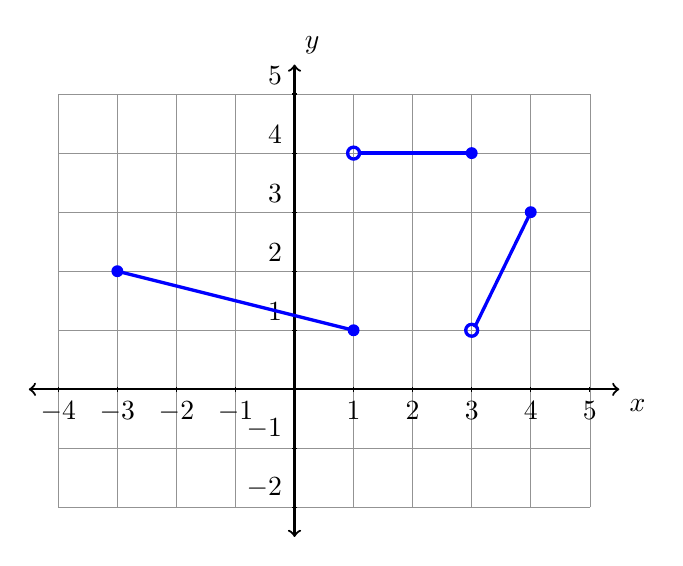
\begin{tikzpicture}[y=.75cm, x=.75cm,font=\sffamily,
	mydot/.style={
    circle,
    fill=white,
    draw,
    outer sep=0pt,
    inner sep=1.5pt
  }]
    %% Add a grid
    \draw[step = 1, gray, very thin,opacity=0.85] (-4, -2) grid (5, 5);
 	%% Draw the axes
	\draw[thick,<->] (-4.5,0) -- coordinate (x axis mid) (5.5,0) node[anchor = north west] {$x$};
    \draw[thick,<->] (0,-2.5) -- coordinate (y axis mid) (0,5.5) node[anchor = south west] {$y$};
    %% Label the y axis
    \foreach \y in {-2,...,-1,1,2,...,5} {
      \draw (1pt, \y) -- (-1pt, \y) node[anchor = south east] {$\y$};
    }
    %% Label the x axis
    \foreach \x in {-4,...,-1,1,2,...,5} {
      \draw (\x,1pt) -- (\x,-1pt) node[anchor = north] {$\x$};
    }
    %% Draw the function.
    \begin{scope}
         \draw[very thick,blue] (-3,2) -- (1,1);
         \draw[very thick,blue] (3.05,1.05) -- (4,3);
         \draw[very thick,blue] (1.1,4) -- (3,4);
    %semi-circle
         %\draw[very thick, blue] (1,1) arc [radius=1, start angle=180, end angle= 5];
     %parabola
     %    \draw[ultra thick, blue, domain=-5:0] plot (\x, {(-0.2)*(\x-5)*(\x+5)});
     %dots
         \fill[blue] (-3, 2) circle[radius=0.5ex];
         \fill[blue] (1,1) circle[radius=0.5ex];
         \fill[blue] (4,3) circle[radius=0.5ex];
         \draw[very thick, blue] (3,1) circle[radius=0.5ex];
         \fill[blue] (3,4) circle[radius=0.5ex];
         \draw[very thick, blue] (1,4) circle[radius=0.5ex];


    \end{scope}

    %%\node[above=0.1cm] at (-2,2 )   {\nextXValue};

\end{tikzpicture}

\vfill

\item \ 

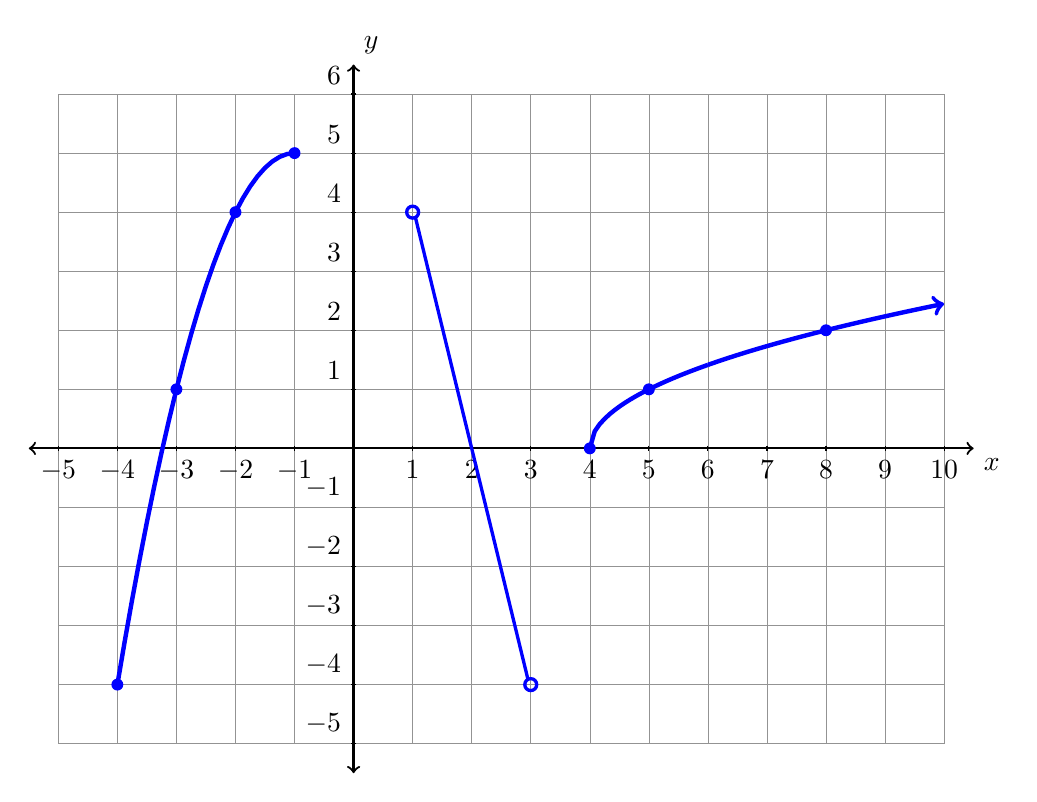
\begin{tikzpicture}[y=.75cm, x=.75cm,font=\sffamily,
	mydot/.style={
    circle,
    fill=white,
    draw,
    outer sep=0pt,
    inner sep=1.5pt
  }]
    %% Add a grid
    \draw[step = 1, gray, very thin,opacity=0.85] (-5, -5) grid (10, 6);
 	%% Draw the axes
	\draw[thick,<->] (-5.5,0) -- coordinate (x axis mid) (10.5,0) node[anchor = north west] {$x$};
    \draw[thick,<->] (0,-5.5) -- coordinate (y axis mid) (0,6.5) node[anchor = south west] {$y$};
    %% Label the y axis
    \foreach \y in {-5,...,-1,1,2,...,6} {
      \draw (1pt, \y) -- (-1pt, \y) node[anchor = south east] {$\y$};
    }
    %% Label the x axis
    \foreach \x in {-5,...,-1,1,2,...,10} {
      \draw (\x,1pt) -- (\x,-1pt) node[anchor = north] {$\x$};
    }
    %% Draw the function.
    \begin{scope}
    %     \draw[very thick,blue] (-3,2) -- (1,1);
       %  \draw[very thick,blue] (3.05,1.05) -- (4,3);
         \draw[very thick,blue] (1.05,3.9) -- (2.95,-3.9);
    %semi-circle
         %\draw[very thick, blue] (1,1) arc [radius=1, start angle=180, end angle= 5];
     %parabola
         \draw[ultra thick, blue, domain=-4:-1] plot (\x, {-(\x+1)^2+5});
         \draw[ultra thick, blue, domain=4:6] plot (\x, {(\x-4)^(1/2)});
         \draw[ultra thick, blue, ->, domain=6:10] plot (\x, {(\x-4)^(1/2)});
     %dots
         \fill[blue] (-4, -4) circle[radius=0.5ex];
         \fill[blue] (-1,5) circle[radius=0.5ex];
         \fill[blue] (-2,4) circle[radius=0.5ex];
         \draw[very thick, blue] (3,-4) circle[radius=0.5ex];
         \fill[blue] (-3,1) circle[radius=0.5ex];
         \fill[blue] (4,0) circle[radius=0.5ex];
         \fill[blue] (5,1) circle[radius=0.5ex];
         \fill[blue] (8,2) circle[radius=0.5ex];

         \draw[very thick, blue] (1,4) circle[radius=0.5ex];


    \end{scope}

    %%\node[above=0.1cm] at (-2,2 )   {\nextXValue};

\end{tikzpicture}

\vfill

\end{enumerate}


\newpage

\item Determine whether or not the following graphs display odd symmetry, even symmetry, or neither.

\begin{multicols}{2}

\begin{enumerate}

\item \ 

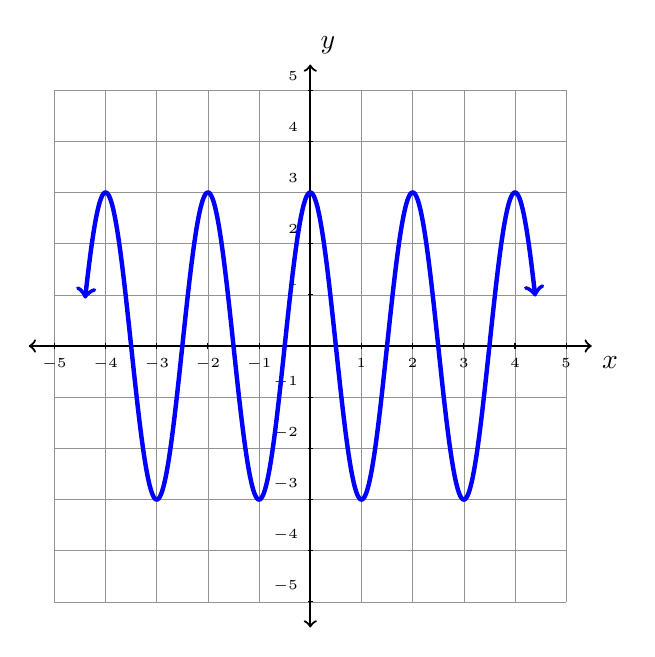
\begin{tikzpicture}[y=.65cm, x=.65cm,font=\sffamily,
	mydot/.style={
    circle,
    fill=white,
    draw,
    outer sep=0pt,
    inner sep=1.5pt
  }]
    %% Add a grid
    \draw[step = 1, gray, very thin,opacity=0.85] (-5, -5) grid (5, 5);
 	%% Draw the axes
	\draw[thick,<->] (-5.5,0) -- coordinate (x axis mid) (5.5,0) node[anchor = north west] {$x$};
    \draw[thick,<->] (0,-5.5) -- coordinate (y axis mid) (0,5.5) node[anchor = south west] {$y$};
    %% Label the y axis
    \foreach \y in {-5,...,-1,1,2,...,5} {
      \draw (1pt, \y) -- (-1pt, \y) node[anchor = south east] {\tiny $\y$};
    }
    %% Label the x axis
    \foreach \x in {-5,...,-1,1,2,...,5} {
      \draw (\x,1pt) -- (\x,-1pt) node[anchor = north] {\tiny $\x$};
    }
    %% Draw the function.
    \begin{scope}
%         \draw[very thick,blue] (-3,2) -- (1,1);
%         \draw[very thick,blue] (3.05,1.05) -- (4,3);
%         \draw[very thick,blue] (1.1,4) -- (3,4);
    %semi-circle
         %\draw[very thick, blue] (1,1) arc [radius=1, start angle=180, end angle= 5];
     %parabola
         %\draw[ultra thick, blue, domain=-5:0] plot (\x, {(-0.2)*(\x-5)*(\x+5)});
         \draw[ultra thick, blue, <->, domain=-4.4:4.4] plot[samples=1000] (\x, {3*cos(pi*\x r)});             %dots
%         \fill[blue] (-3, 2) circle[radius=0.5ex];
%         \fill[blue] (1,1) circle[radius=0.5ex];
%         \fill[blue] (4,3) circle[radius=0.5ex];
%         \draw[very thick, blue] (3,1) circle[radius=0.5ex];
%         \fill[blue] (3,4) circle[radius=0.5ex];
%         \draw[very thick, blue] (1,4) circle[radius=0.5ex];


    \end{scope}

    %%\node[above=0.1cm] at (-2,2 )   {\nextXValue};

\end{tikzpicture}

\item \ 


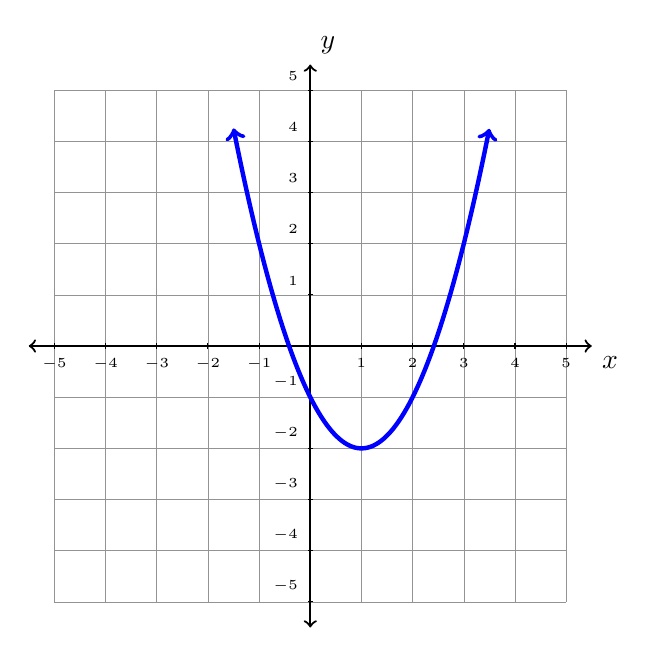
\begin{tikzpicture}[y=.65cm, x=.65cm,font=\sffamily,
	mydot/.style={
    circle,
    fill=white,
    draw,
    outer sep=0pt,
    inner sep=1.5pt
  }]
    %% Add a grid
    \draw[step = 1, gray, very thin,opacity=0.85] (-5, -5) grid (5, 5);
 	%% Draw the axes
	\draw[thick,<->] (-5.5,0) -- coordinate (x axis mid) (5.5,0) node[anchor = north west] {$x$};
    \draw[thick,<->] (0,-5.5) -- coordinate (y axis mid) (0,5.5) node[anchor = south west] {$y$};
    %% Label the y axis
    \foreach \y in {-5,...,-1,1,2,...,5} {
      \draw (1pt, \y) -- (-1pt, \y) node[anchor = south east] {\tiny $\y$};
    }
    %% Label the x axis
    \foreach \x in {-5,...,-1,1,2,...,5} {
      \draw (\x,1pt) -- (\x,-1pt) node[anchor = north] {\tiny $\x$};
    }
    %% Draw the function.
    \begin{scope}
%         \draw[very thick,blue] (-3,2) -- (1,1);
%         \draw[very thick,blue] (3.05,1.05) -- (4,3);
%         \draw[very thick,blue] (1.1,4) -- (3,4);
    %semi-circle
         %\draw[very thick, blue] (1,1) arc [radius=1, start angle=180, end angle= 5];
     %parabola
         %\draw[ultra thick, blue, domain=-5:0] plot (\x, {(-0.2)*(\x-5)*(\x+5)});
         \draw[ultra thick, blue, <->, domain=-1.5:3.5] plot[samples=100] (\x, {(\x-1)^2-2});
           %dots
%         \fill[blue] (-3, 2) circle[radius=0.5ex];
%         \fill[blue] (1,1) circle[radius=0.5ex];
%         \fill[blue] (4,3) circle[radius=0.5ex];
%         \draw[very thick, blue] (3,1) circle[radius=0.5ex];
%         \fill[blue] (3,4) circle[radius=0.5ex];
%         \draw[very thick, blue] (1,4) circle[radius=0.5ex];


    \end{scope}

    %%\node[above=0.1cm] at (-2,2 )   {\nextXValue};

\end{tikzpicture}

\columnbreak

\item \ 

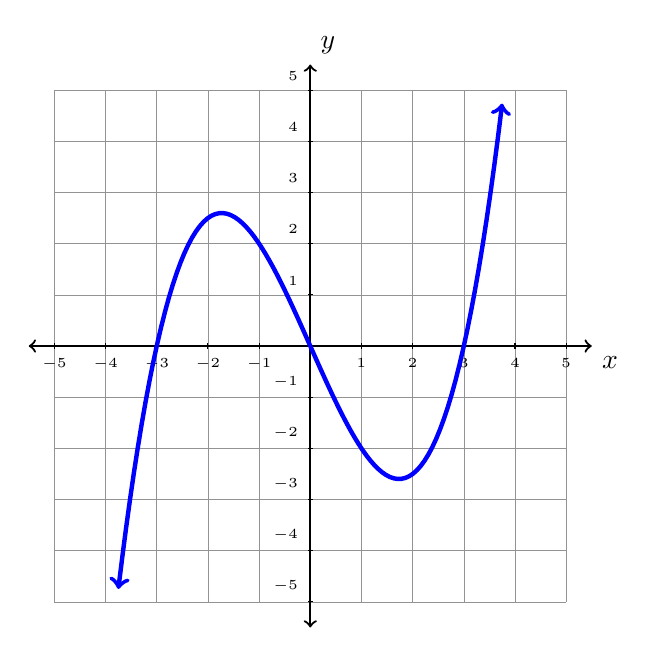
\begin{tikzpicture}[y=.65cm, x=.65cm,font=\sffamily,
	mydot/.style={
    circle,
    fill=white,
    draw,
    outer sep=0pt,
    inner sep=1.5pt
  }]
    %% Add a grid
    \draw[step = 1, gray, very thin,opacity=0.85] (-5, -5) grid (5, 5);
 	%% Draw the axes
	\draw[thick,<->] (-5.5,0) -- coordinate (x axis mid) (5.5,0) node[anchor = north west] {$x$};
    \draw[thick,<->] (0,-5.5) -- coordinate (y axis mid) (0,5.5) node[anchor = south west] {$y$};
    %% Label the y axis
    \foreach \y in {-5,...,-1,1,2,...,5} {
      \draw (1pt, \y) -- (-1pt, \y) node[anchor = south east] {\tiny $\y$};
    }
    %% Label the x axis
    \foreach \x in {-5,...,-1,1,2,...,5} {
      \draw (\x,1pt) -- (\x,-1pt) node[anchor = north] {\tiny $\x$};
    }
    %% Draw the function.
    \begin{scope}
%         \draw[very thick,blue] (-3,2) -- (1,1);
%         \draw[very thick,blue] (3.05,1.05) -- (4,3);
%         \draw[very thick,blue] (1.1,4) -- (3,4);
    %semi-circle
         %\draw[very thick, blue] (1,1) arc [radius=1, start angle=180, end angle= 5];
     %parabola
         %\draw[ultra thick, blue, domain=-5:0] plot (\x, {(-0.2)*(\x-5)*(\x+5)});
         \draw[ultra thick, blue, <->, domain=-3.75:3.75] plot[samples=100] (\x, {(.25)*(\x-3)*(\x)*(\x+3)});
           %dots
%         \fill[blue] (-3, 2) circle[radius=0.5ex];
%         \fill[blue] (1,1) circle[radius=0.5ex];
%         \fill[blue] (4,3) circle[radius=0.5ex];
%         \draw[very thick, blue] (3,1) circle[radius=0.5ex];
%         \fill[blue] (3,4) circle[radius=0.5ex];
%         \draw[very thick, blue] (1,4) circle[radius=0.5ex];


    \end{scope}

    %%\node[above=0.1cm] at (-2,2 )   {\nextXValue};

\end{tikzpicture}

\item \ 

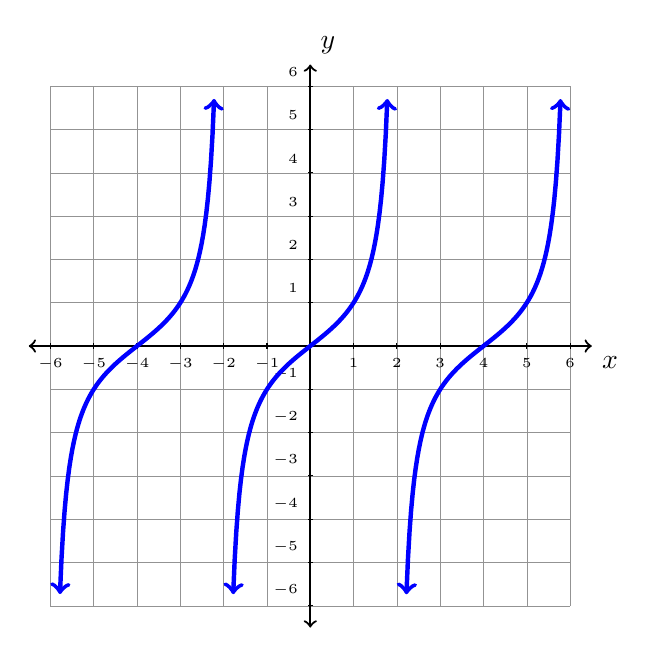
\begin{tikzpicture}[y=.55cm, x=.55cm,font=\sffamily,
	mydot/.style={
    circle,
    fill=white,
    draw,
    outer sep=0pt,
    inner sep=1.5pt
  }]
    %% Add a grid
    \draw[step = 1, gray, very thin,opacity=0.85] (-6, -6) grid (6, 6);
 	%% Draw the axes
	\draw[thick,<->] (-6.5,0) -- coordinate (x axis mid) (6.5,0) node[anchor = north west] {$x$};
    \draw[thick,<->] (0,-6.5) -- coordinate (y axis mid) (0,6.5) node[anchor = south west] {$y$};
    %% Label the y axis
    \foreach \y in {-6,...,-1,1,2,...,6} {
      \draw (1pt, \y) -- (-1pt, \y) node[anchor = south east] {\tiny $\y$};
    }
    %% Label the x axis
    \foreach \x in {-6,...,-1,1,2,...,6} {
      \draw (\x,1pt) -- (\x,-1pt) node[anchor = north] {\tiny $\x$};
    }
    %% Draw the function.
    \begin{scope}
%         \draw[very thick,blue] (-3,2) -- (1,1);
%         \draw[very thick,blue] (3.05,1.05) -- (4,3);
%         \draw[very thick,blue] (1.1,4) -- (3,4);
    %semi-circle
         %\draw[very thick, blue] (1,1) arc [radius=1, start angle=180, end angle= 5];
     %parabola
         %\draw[ultra thick, blue, domain=-5:0] plot (\x, {(-0.2)*(\x-5)*(\x+5)});
         \draw[ultra thick, blue, <->, domain=-1.78:1.78] plot[samples=100] (\x, {tan(.25*pi*\x r)});
         \draw[ultra thick, blue, <->, domain=-5.78:-2.22] plot[samples=100] (\x, {tan(.25*pi*\x r)});
         \draw[ultra thick, blue, <->, domain=2.22:5.78] plot[samples=100] (\x, {tan(.25*pi*\x r)});
           %dots
%         \fill[blue] (-3, 2) circle[radius=0.5ex];
%         \fill[blue] (1,1) circle[radius=0.5ex];
%         \fill[blue] (4,3) circle[radius=0.5ex];
%         \draw[very thick, blue] (3,1) circle[radius=0.5ex];
%         \fill[blue] (3,4) circle[radius=0.5ex];
%         \draw[very thick, blue] (1,4) circle[radius=0.5ex];


    \end{scope}

    %%\node[above=0.1cm] at (-2,2 )   {\nextXValue};

\end{tikzpicture}


\end{enumerate}



\end{multicols}

%\vfill
%
%\item Find a function that is both even and odd.



\clearpage

\item The domain of an even function, $A(x)$, is all real numbers. For
  positive values of $x$ the value of $A(x)$ is equal to $x$.
  \label{question:1.7:absoluteValue}
  \begin{enumerate}
  \item Make a sketch of the function $A(x)$ for $-3\leq x \leq 3$.
    \vfill
    \vfill
  \item Determine a formula for the function if $x$ is negative.
    \vfill
  \item Express the function $A(x)$ as a piecewise defined function.
    \vfill
  \item Express the function $A(x)$ in terms of another, basic
    function.
    \vfill
  \item Determine the values of $x$ where $A(x)$ is increasing and the
    values where $A(x)$ is decreasing.
    \vfill
  \end{enumerate}

%\newpage 
%\item Use the graph of $y=f(x)$ to answer the following questions.
%\begin{center}
%	\begin{tikzpicture}[y=1cm, x=1cm,font=\sffamily,
%	mydot/.style={
%    circle,
%    fill=white,
%    draw,
%    outer sep=0pt,
%    inner sep=1.5pt
%  }]
%    %% Add a grid
%    \draw[step = 1, gray, very thin,opacity=0.85] (-6, -2) grid (6, 6);
% 	%% Draw the axes
%	\draw[thick,<->] (-6.5,0) -- coordinate (x axis mid) (6.5,0) node[anchor = north west] {$x$};
%    \draw[thick,<->] (0,-2.5) -- coordinate (y axis mid) (0,6.5) node[anchor = south west] {$y$};
%    %% Label the y axis
%    \foreach \y in {-2,...,-1,1,2,...,6} {
%      \draw (1pt, \y) -- (-1pt, \y) node[anchor = south east] {$\y$};
%    }
%    %% Label the x axis
%    \foreach \x in {-6,...,-1,1,2,...,6} {
%      \draw (\x,1pt) -- (\x,-1pt) node[anchor = north] {$\x$};
%    }
%    %% Draw the function.
%    \begin{scope}
%         \draw[very thick,blue] (-3,2) -- (1,1);
%         \draw[very thick,blue] (3.05,1.05) -- (4,3);
%    %semi-circle
%         \draw[very thick, blue] (1,1) arc [radius=1, start angle=180, end angle= 5];
%     %parabola
%     %    \draw[ultra thick, blue, domain=-5:0] plot (\x, {(-0.2)*(\x-5)*(\x+5)});
%     %dots
%         \fill[blue] (-3, 2) circle[radius=0.5ex];
%         \fill[blue] (1,1) circle[radius=0.5ex];
%         \fill[blue] (4,3) circle[radius=0.5ex];
%         \draw[very thick, blue] (3,1) circle[radius=0.5ex];
%
%
%    \end{scope}
%
%    %%\node[above=0.1cm] at (-2,2 )   {\nextXValue};
%
%  \end{tikzpicture}
%\end{center}
%
%
%\begin{enumerate}
%\item Determine the intervals where $f(x)$ is increasing.\vfill
%\item Determine the intervals where $f(x)$ is decreasing.\vfill
%\item Determine the \textbf{location} of any relative minima.\vfill
%\item Determine the \textbf{value} of any relative minima.\vfill
%\item Determine the \textbf{location} of any relative maxima.\vfill
%\item Determine the \textbf{value} of any relative maxima.\vfill
%\end{enumerate}



\end{enumerate}

\hwTitle{Section 1.7}

\begin{enumerate}
\item Complete question \ref{question:1.7:absoluteValue}.
\item A store sells cold drinks. From 10:00am till 12:00pm (noon) it
  sells 0.2 drinks per minute. From 12:00pm till 4:00pm it sells 0.4
  drinks per minute. Determine the function that gives the number of
  drinks sold in one day given the number of minutes past 10:00am.
  State your final answer as a function of time and as a piecewise
  defined function.

\item The graph of a function, $h(x)$, is given below. Use the graph
  to answer each of the questions below.

    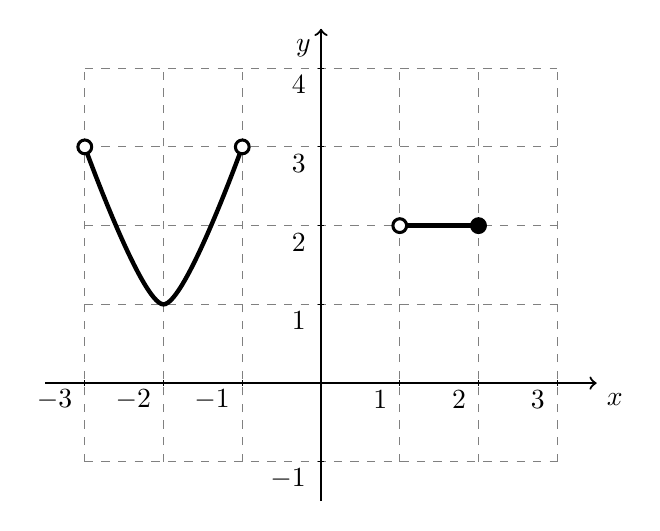
\begin{tikzpicture}[y=1.0cm, x=1.0cm,font=\sffamily]
        %% ticks
        \draw[step = 1, gray,dashed] (-3,-1) grid (3,4);
        %% axis
        \draw[thick,->] (-3.5,0) -- coordinate (x axis mid) (3.5,0) node[anchor = north west] {$x$};
        \draw[thick,->] (0,-1.5) -- coordinate (y axis mid) (0,4.5) node[anchor = north east] {$y$};
        \foreach \y in {-1,1,2,3,4} {
          \draw (1pt, \y) -- (-1pt, \y) node[yshift=-6,xshift=-1,anchor=east] {$\y$};
        }
        \foreach \x in {-3,-2,-1,1,2,3} {
          \draw (\x,1pt) -- (\x,-1pt) node[yshift=-5,xshift=-1,anchor=east] {$\x$};
        }

        \draw[ultra thick] plot [smooth] coordinates
           {(-3,3) (-2,1) (-1,3)};

        \draw[ultra thick] plot [smooth] coordinates
           {(1,2) (2,2) };
        
        %\draw[ultra thick,black]
        % (-4, 0) .. controls +(35: 1) and +(180:0.5) .. (-2, 2)
        % (-2, 2) .. controls +(0:0.5) and +(135:1)   .. (0, 0);
        % (-2, 0) .. controls +( 90:0.5) and +(-40:-0.5) .. (0,3)
        % ( 0, 3) .. controls +(-40:0.5) and +(-15:-1) .. (3, 2);

        % \draw[ultra thick,black] (0,-1) --  (4,3);
        \draw[black,fill=black]  (-3,3) circle (0.1);
        \draw[black,fill=white]  (-3,3) circle (0.075);
        \draw[black,fill=black]  (-1,3) circle (0.1);
        \draw[black,fill=white]  (-1,3) circle (0.075);
        \draw[black,fill=black]  (1,2) circle (0.1);
        \draw[black,fill=white]  (1,2) circle (0.075);
        \draw[black,fill=black]  (2,2) circle (0.1);
      \end{tikzpicture}



    \begin{enumerate}
    \item Determine the domain and range of $h(x)$.
    \item Determine the intervals where the function is
      increasing and the intervals where the function is decreasing.
    \item Determine the formula for the function using
      proper notation for a piecewise defined function. (The curved
      part to the left is a parabola.)
    \end{enumerate}

\item The cost to use a parking garage is \$5.00 for the first
    thirty minutes. After thirty minutes the cost is an additional
    five cents for each minute thereafter.
    \begin{enumerate}
    \item Determine the formula for the cost to park a car given the
      number of minutes it is parked and use proper notation for a
      piecewise defined function.
    \item Determine the average rate of change of the cost to park a
      car between $t$ minutes and zero minutes. (In other words what
      is the average rate of change of the cost from time $t$ to time
      0.) What happens to the average rate of change after a very long
      time?
    \end{enumerate}

\end{enumerate}
